\documentclass[12pt,a4paper]{article}
\usepackage{amsmath,amssymb}
\usepackage{graphicx}
\usepackage{geometry}
\usepackage{float}
\usepackage{booktabs}
\usepackage{xcolor}
\usepackage{hyperref}

\usepackage{xepersian}

\settextfont{B-NAZANIN.TTF} 
\setlatintextfont[Scale=0.85]{Times New Roman}

\renewcommand{\labelitemi}{$\bullet$}
\renewcommand{\labelitemii}{$\circ$}

\title{گزارش پروژه دوم بینایی سه‌بعدی و کالیبراسیون دوربین}
\author{استاد درس:‌ دکتر جوانمردی، دکتر خادمیان \\ امیررضا کاظم لو \\ \small درس ربات های متحرک خودگردان \\}
\date{\today}

\begin{document}
\maketitle

\section{مقدمه و آماده‌سازی}
برای این که کالیبریشن انجام شود ما به صفحه شطرنجی (\lr{Chessboard}) نیاز داشتیم که از سایت \lr{https://calib.io/pages/camera-calibration-pattern-generator} تهیه شد که در فایل \textbf{\lr{calib.io\_checker\_200x150\_8x11\_15.pdf}} قرار گرفته است و سپس آن را در صفحه نمایش کامپیوتر نمایش داده شده است و از زوایای مختلف و فاصله‌های مختلف تصویربرداری شده است. نکته مهم در تصویری که در زیر مشخص شده است:

\begin{figure}[H]
    \centering
    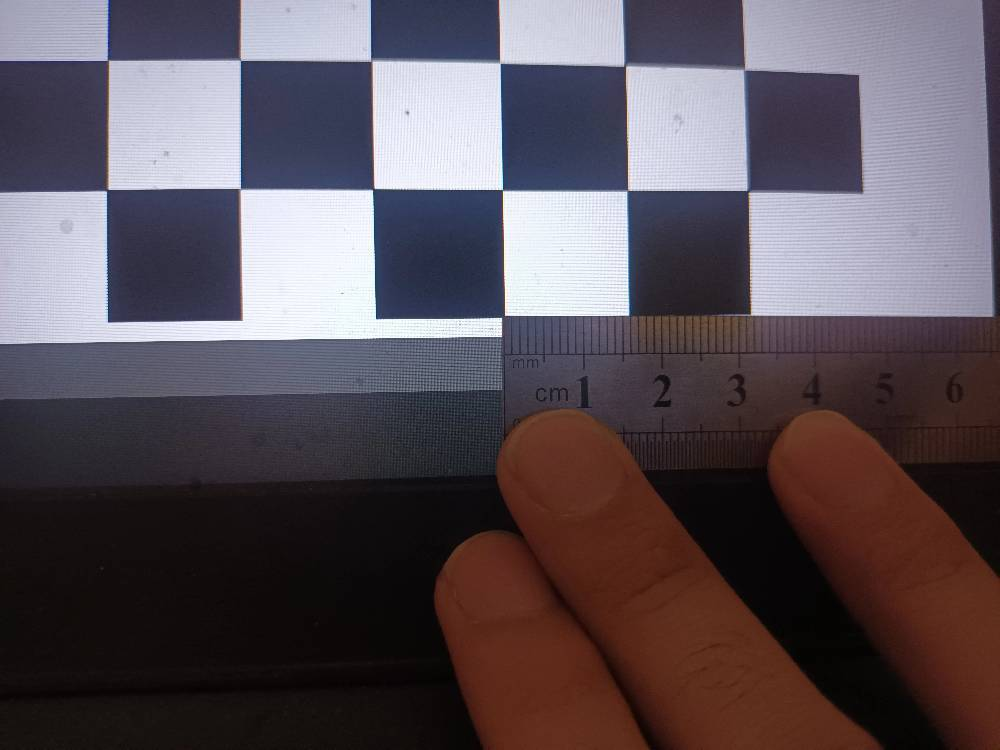
\includegraphics[width=0.6\textwidth]{./images/clarification the size of each square.jpg}
    \caption{بررسی ابعاد مربع‌های صفحه کالیبراسیون}
\end{figure}

اندازه هر کدام از مربع‌ها برابر ۱۶ میلی‌متر است و این مبنای ما در تبدیل فضای سه‌بعدی به دوبعدی و محاسبه ماتریس درونی و بیرونی دوربین می‌باشد.
در بخشی از این تمرین، باید مقدار متغیر \lr{\texttt{square\_size\_mm}} تعیین می‌شد. واحد اندازه‌گیری اختصاص‌یافته به این متغیر، مستقیماً واحد خروجی‌های سیستم را تعیین می‌کند؛ بدین معنا که اگر این ابعاد بر حسب متر تعریف شوند، خروجی‌ها نیز بر حسب متر خواهند بود و اگر میلی‌متر انتخاب شود، نتایج نیز میلی‌متری محاسبه می‌شوند. در کدهای پیاده‌سازی‌شده، این مقدار بر حسب متر (یعنی $0.016$) لحاظ شده است.

نکته مهم دیگری که در کلاس درس نیز به آن اشاره شد، تفاوت پردازش صفحات شطرنجی (\lr{Chessboard}) معمولی با نمونه‌های علامت‌گذاری‌شده (مانند الگوهای دارای گراف و کدهای اطلاعاتی) است. در صفحات شطرنجی استاندارد و بدون علامت، ضروری است که تمام صفحه در کادر تصویر مشخص باشد؛ در غیر این صورت، توابع \lr{OpenCV} آن تصویر را نادیده می‌گیرند. دلیل این محدودیت این است که مبدأ دستگاه مختصات جهانی در گوشه این صفحات در نظر گرفته می‌شود و با ناقص بودن تصویر، این مبدأ گم می‌شود. در مقابل، در نمونه‌های علامت‌گذاری‌شده، سیستم می‌تواند به کمک همان شناسه‌ها و نشانه‌های بصری، موقعیت دقیق هر خانه از صفحه شطرنجی را حتی در صورت رؤیت‌پذیر نبودن کل صفحه، به درستی تشخیص دهد.

\section{مبانی تئوری کالیبراسیون دوربین}
در فرآیند کالیبراسیون، هدف برقراری یک رابطه ریاضی دقیق بین مختصات نقاط در دنیای سه‌بعدی و پیکسل‌های متناظر آن‌ها در تصویر دوبعدی است. برای این منظور از مدل دوربین سوراخ‌سوزنی (\lr{Pinhole Camera Model}) استفاده می‌شود.

\subsection{ماتریس درونی (\lr{Intrinsic Matrix})}
ماتریس درونی شامل پارامترهایی است که به ساختار داخلی خود دوربین بستگی دارند. این پارامترها شامل فاصله کانونی (\lr{Focal Length}) و مختصات نقطه اصلی (\lr{Principal Point}) در صفحه تصویر هستند. ماتریس درونی $K$ به فرم زیر تعریف می‌شود:
\begin{equation}
K = \begin{bmatrix} f_x & 0 & c_x \\ 0 & f_y & c_y \\ 0 & 0 & 1 \end{bmatrix}
\end{equation}
که در آن $f_x$ و $f_y$ فاصله‌های کانونی بر حسب پیکسل، و $c_x$ و $c_y$ مختصات مرکز نوری تصویر می‌باشند.

\subsection{ماتریس بیرونی (\lr{Extrinsic Matrix})}
ماتریس بیرونی نشان‌دهنده موقعیت و جهت‌گیری دوربین در فضای سه‌بعدی نسبت به یک دستگاه مختصات مرجع (جهانی) است. این انتقال با یک ماتریس دوران (\lr{Rotation Matrix}) ۳ در ۳ که با $R$ نشان داده می‌شود و یک بردار انتقال (\lr{Translation Vector}) ۳ در ۱ که با $T$ نشان داده می‌شود، بیان می‌گردد. 

رابطه کلی تصویر کردن یک نقطه سه‌بعدی در مختصات جهانی $M=[X, Y, Z, 1]^T$ به یک نقطه دوبعدی $m=[u, v, 1]^T$ در صفحه تصویر به صورت زیر است:
\begin{equation}
s m = K [R | T] M
\end{equation}
که در آن $s$ یک ضریب مقیاس (\lr{Scale Factor}) است.

\subsection{تکنیک کالیبراسیون ژانگ (\lr{Zhang's Method}) و مبنای هندسه دوبعدی}
روش‌های سنتی کالیبراسیون دوربین نیازمند یک شیء سه‌بعدی با ساختار کارگاهی بسیار دقیق و گران‌قیمت بودند تا بتوانند مختصات سه‌بعدی واقعی نقاط کنترل را با پیکسل‌های دوبعدی متناظر در تصویر هم‌راستا کنند. فرآیند کالیبراسیون با روش ژانگ (\lr{Zhang's Method}) به جای اشیای سه‌بعدی پیچیده، تنها از یک صفحه مسطح دوبعدی (مانند الگوی شطرنجی یا \lr{Chessboard}) که از زوایای مختلف تصویربرداری شده است، استفاده می‌کند.

مبنای ریاضی این روش بر پایه مفهوم ماتریس هموگرافی (\lr{Homography Matrix}) استوار است. اگر فرض کنیم صفحه شطرنجی کالیبراسیون روی صفحه $Z=0$ در دستگاه مختصات جهانی قرار دارد، هر نقطه سه‌بعدی روی الگو به صورت $M=[X,Y,0,1]^T$ ساده‌سازی می‌شود. با جایگذاری این فرض در معادله پروجکشن دوربین، رابطه پرسپکتیو به صورت زیر بازنویسی می‌گردد:
\begin{equation}
	sm = K\begin{bmatrix}r_1 & r_2 & r_3 & t\end{bmatrix}\begin{bmatrix}X \\ Y \\ 0 \\ 1\end{bmatrix} = K\begin{bmatrix}r_1 & r_2 & t\end{bmatrix}\begin{bmatrix}X \\ Y \\ 1\end{bmatrix}
\end{equation}
در این رابطه، $r_1$، $r_2$ و $r_3$ ستون‌های ماتریس دوران $R$ هستند. ماتریس هموگرافی $H$ به صورت یک ماتریس $3\times3$ تعریف می‌شود که صفحه دوبعدی الگو را مستقیماً به صفحه تصویر نگاشت می‌کند:
\begin{equation}
	H = K\begin{bmatrix}r_1 & r_2 & t\end{bmatrix} = \begin{bmatrix}h_1 & h_2 & h_3\end{bmatrix}
\end{equation}
بنابراین معادله پروجکشن به فرم ساده $sm = HM'$ تبدیل می‌شود که در آن $M'=[X,Y,1]^T$ است. ماتریس هموگرافی $H$ را می‌توان به ازای هر تصویر با داشتن حداقل ۴ تناظر نقطه‌ای بین صفحه شطرنجی واقعی و تصویر استخراج کرد.
هر نمای مستقل از صفحه شطرنجی، یک ماتریس هموگرافی جدید و در نتیجه دو معادله مستقل فوق را فراهم می‌سازد. از آنجا که ماتریس درونی $K$ دارای ۵ پارامتر مجهول است، با داشتن حداقل ۳ تصویر متمایز از صفحه شطرنجی در زوایا و چرخش‌های مختلف، می‌توان این دستگاه معادلات را به روش کمترین مربعات خطی حل نمود و پارامترهای درونی دوربین را بدون نیاز به هیچ‌گونه مانیپولاتور یا ساختار سه‌بعدی پیش‌فرض استخراج کرد.

\subsection{اعوجاج لنز (\lr{Lens Distortion})}
در دوربین‌های واقعی به دلیل شکل کروی لنزها، نقص‌هایی در تصویرسازی رخ می‌دهد که به آن اعوجاج می‌گویند. دو نوع اصلی اعوجاج عبارتند از:
\begin{enumerate}
    \item \textbf{اعوجاج شعاعی (\lr{Radial Distortion}):} باعث می‌شود خطوط مستقیم در لبه‌های تصویر خمیده به نظر برسند. معادلات تصحیح آن به صورت زیر است:
    \begin{align}
    x_{corrected} &= x(1 + k_1 r^2 + k_2 r^4 + k_3 r^6) \\
    y_{corrected} &= y(1 + k_1 r^2 + k_2 r^4 + k_3 r^6)
    \end{align}
    که در آن $r^2=x^2+y^2$ می‌باشد. برای لنزهایی با اعوجاج کم می‌توان از $k_3$ صرف‌نظر کرد.
    
    \item \textbf{اعوجاج مماسی (\lr{Tangential Distortion}):} ناشی از عدم توازی کامل لنز با صفحه سنسور تصویر در فرآیند ساخت است. روابط آن عبارت است از:
    \begin{align}
    x_{corrected} &= x + [2p_1xy + p_2(r^2 + 2x^2)] \\
    y_{corrected} &= y + [p_1(r^2 + 2y^2) + 2p_2xy]
    \end{align}
\end{enumerate}

\section{پیاده‌سازی و استخراج پارامترها}
پیاده‌سازی فرآیند کالیبراسیون با استفاده از زبان \lr{Python} و توابع کتابخانه \lr{OpenCV} انجام گردید. مراحل کار به این صورت بود که ابتدا تمامی تصاویر کالیبراسیون (شامل صفحه شطرنجی با ۱۰ در ۷ گوشه داخلی) بارگذاری شده و به مقیاس خاکستری تبدیل گردیدند. 
برای یافتن گوشه‌ها از تابع \lr{cv2.findChessboardCorners} استفاده شد و به منظور افزایش دقت محاسبه مختصات گوشه‌ها در حد زیرپیکسل (\lr{Sub-pixel Accuracy})، تابع \lr{cv2.cornerSubPix} به کار گرفته شد.
پس از استخراج نقاط در فضای تصویر (\lr{Image Points}) و ایجاد متناظر آن‌ها در فضای سه‌بعدی (\lr{Object Points} با احتساب ابعاد ۱۶ میلی‌متری مربع‌ها)، از تابع \lr{cv2.calibrateCamera} استفاده گردید. خروجی این تابع شامل ماتریس درونی، ضرایب اعوجاج، و بردارهای دوران ($rvecs$) و انتقال ($tvecs$) برای تک‌تک تصاویر است.



\subsection{تشخیص گوشه‌ها در تصاویر الگو}
در گام نخست، الگوی شطرنجی در تصاویر ورودی شناسایی شد. شکل‌های زیر نمونه‌ای از تصویر خام کالیبراسیون و خروجی الگوریتم تشخیص گوشه (\lr{Corner Detection}) را نشان می‌دهند. نقاط یافت شده با استفاده از توابع \lr{OpenCV} با دقت زیرپیکسل (\lr{Sub-pixel}) بهینه‌سازی شدند تا خطای محاسبات به حداقل برسد.

\begin{figure}[H]
	\centering
	\begin{minipage}{0.48\textwidth}
		\centering
		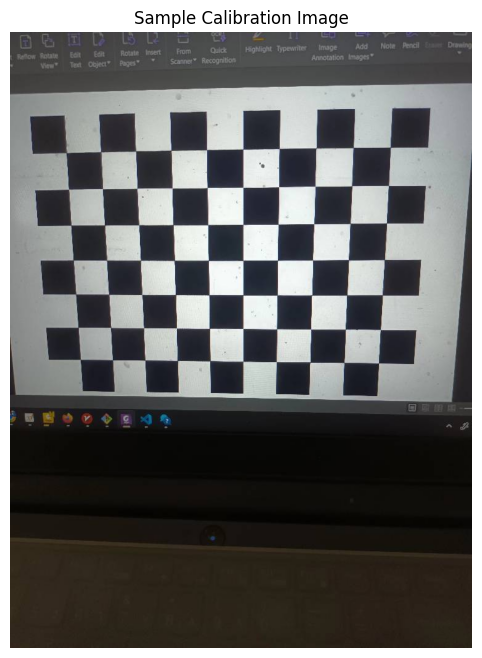
\includegraphics[width=\linewidth]{images/Sample Calibration Image.png}
		\caption{نمونه تصویر خام کالیبراسیون}
	\end{minipage}\hfill
	\begin{minipage}{0.48\textwidth}
		\centering
		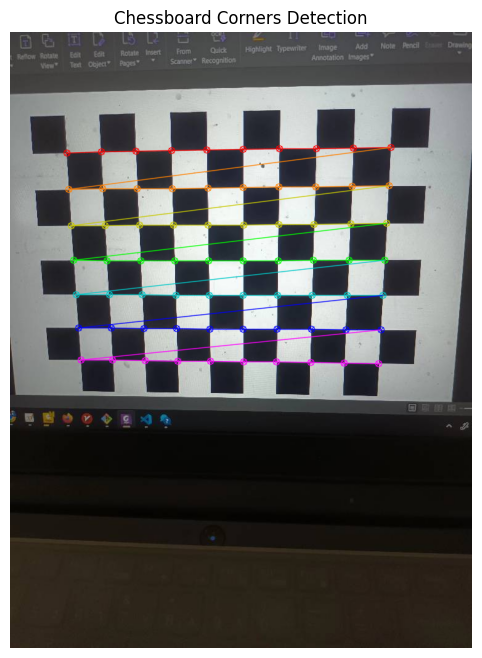
\includegraphics[width=\linewidth]{images/Chessboard Corners Detection.png}
		\caption{تشخیص گوشه‌های صفحه شطرنجی}
	\end{minipage}
\end{figure}

\subsection{ماتریس درونی و ضرایب اعوجاج به دست آمده}
پس از اعمال الگوریتم کالیبراسیون بر روی مجموعه تصاویر، خطای کلی کالیبراسیون (\lr{RMS Error}) برابر با $0.3908$ پیکسل به دست آمد که نشان‌دهنده دقت بالای فرآیند است. 
ماتریس درونی دوربین (\lr{Camera Matrix}) به شکل زیر محاسبه گردید:
\begin{equation}
	K = \begin{bmatrix} 760.91 & 0 & 368.09 \\ 0 & 759.66 & 507.62 \\ 0 & 0 & 1 \end{bmatrix}
\end{equation}
تفسیر این ماتریس نشان می‌دهد که فاصله کانونی (\lr{Focal Length}) در راستای محورهای $x$ و $y$ به ترتیب $760.91$ و $759.66$ پیکسل است. همچنین مختصات نقطه اصلی (\lr{Principal Point}) در تصویر برابر با $(368.09, 507.62)$ می‌باشد.

ضرایب اعوجاج (\lr{Distortion Coefficients}) لنز نیز به صورت زیر استخراج شدند:
\begin{itemize}
	\item \textbf{اعوجاج شعاعی (\lr{Radial Distortion}):} $k_1 = 0.0910$, $k_2 = -0.1990$, $k_3 = -0.2314$
	\item \textbf{اعوجاج مماسی (\lr{Tangential Distortion}):} $p_1 = -0.0017$, $p_2 = 0.0001$
\end{itemize}

\begin{figure}[H]
	\centering
	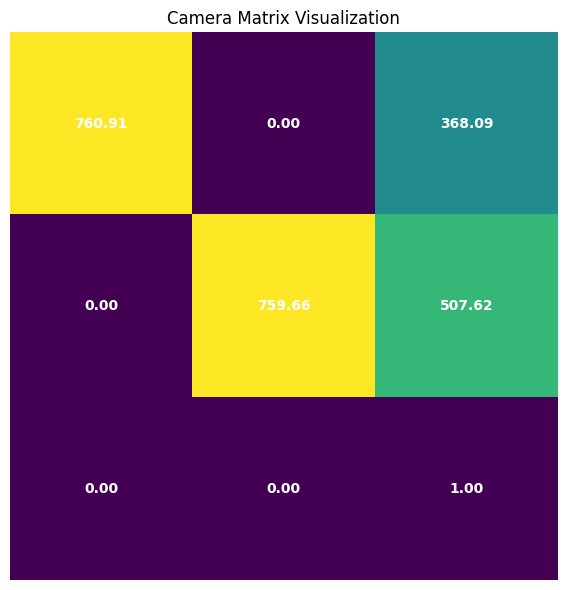
\includegraphics[width=0.7\textwidth]{images/Interpretation of the camera matrix.png}
	\caption{نمایش بصری پارامترهای ماتریس درونی دوربین}
\end{figure}


\subsection{تحلیل حذف اعوجاج (\lr{Undistortion})}
با استفاده از ماتریس درونی و ضرایب اعوجاج محاسبه شده، توانستیم اثرات اعوجاج لنز را از تصاویر حذف کنیم. شکل زیر مقایسه تصویر قبل و بعد از اصلاح اعوجاج را نشان می‌دهد. همان‌طور که مشاهده می‌شود، انحنای خطوط که ناشی از نقص شعاعی لنز بوده، پس از اعمال اصلاحات به خوبی برطرف شده است.

\begin{figure}[H]
	\centering
	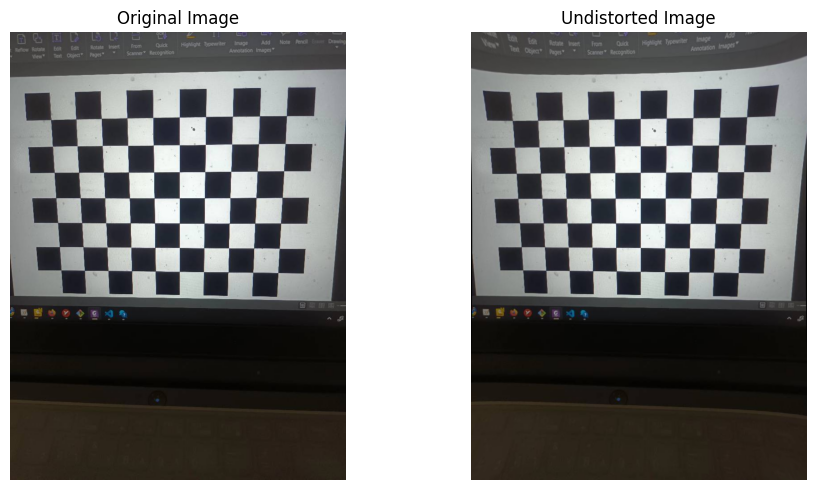
\includegraphics[width=0.8\textwidth]{images/Undistortion Analysis.png}
	\caption{تحلیل و مقایسه تصویر قبل و بعد از حذف اعوجاج}
\end{figure}


\subsection{تحلیل خطای بازتولید (\lr{Reprojection Error})}
برای ارزیابی دقیق‌تر کیفیت کالیبراسیون، خطای بازتولید برای نقاط محاسبه گردید. نتایج آماری این خطا به شرح زیر است:
\begin{itemize}
	\item کمترین میزان خطا: $0.00519$ پیکسل
	\item بیشترین میزان خطا: $2.03520$ پیکسل
	\item میانه خطا (\lr{Median}): $0.26353$ پیکسل
\end{itemize}

\begin{figure}[H]
	\centering
	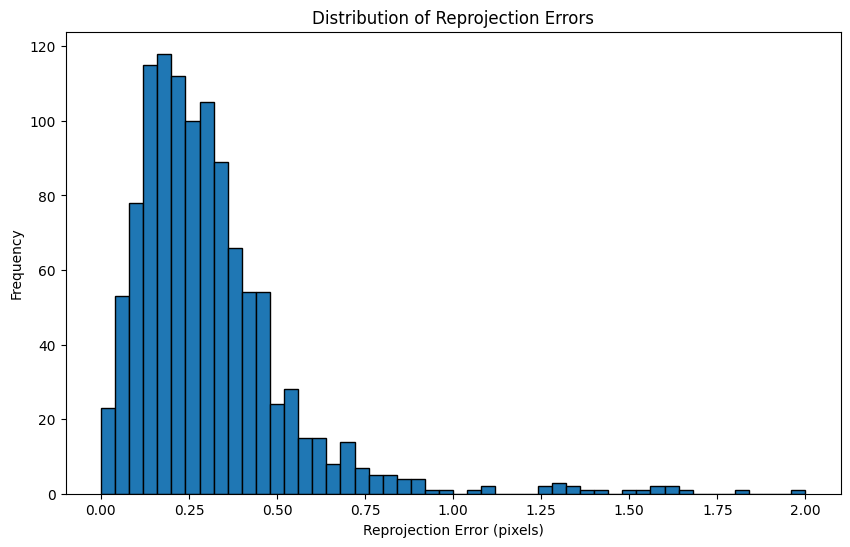
\includegraphics[width=0.7\textwidth]{images/Distribution of Reprojection Errors.png}
	\caption{توزیع خطای بازتولید در تصاویر کالیبراسیون}
\end{figure}

بر اساس نمودار توزیع خطا و مقادیر به دست آمده، می‌توان تفسیر زیر را از نتایج ارائه داد:
\begin{enumerate}
	\item میانگین خطای بازتولید (که کمتر از ۱ پیکسل است) نشان می‌دهد که کالیبراسیون با کیفیت و دقت خوبی انجام شده است.
	\item توزیع خطاها تقریباً از یک توزیع گاوسی (\lr{Gaussian Distribution}) پیروی می‌کند که حول مقادیر نزدیک به صفر متمرکز شده است. این امر نشان‌دهنده عدم وجود خطای سیستماتیک جدی در فرآیند است.
	\item وجود داده‌های پرت (\lr{Outliers}) در توزیع (مواردی که خطای نزدیک به ۲ پیکسل دارند) ممکن است به دلیل تار بودن تصویر (\lr{Motion Blur}) یا استخراج نادرست گوشه‌ها در چند تصویر محدود از مجموعه دادگان باشد.
	\item در مجموع با توجه به پایین بودن خطا، نیازی به تصویربرداری مجدد نیست. با این حال، در صورت نیاز به بهبود فرآیند، می‌توان تصاویری که بیشترین خطا را تولید کرده‌اند شناسایی کرده و از فرآیند کالیبراسیون کنار گذاشت.
\end{enumerate}

\section{نتایج و تفسیر موقعیت‌های سه‌بعدی دوربین}
به منظور درک بهتر هندسه مسئله و بررسی صحت توزیع تصاویر، موقعیت دوربین در زمان ثبت هر تصویر نسبت به صفحه کالیبراسیون مدل‌سازی شد. با استفاده از کتابخانه \lr{Matplotlib}، مختصات مرکز دوربین در سیستم مختصات جهانی (که صفحه شطرنجی در صفحه $Z=0$ آن قرار دارد) به دست آمد و رسم گردید.

\begin{figure}[H]
	\centering
	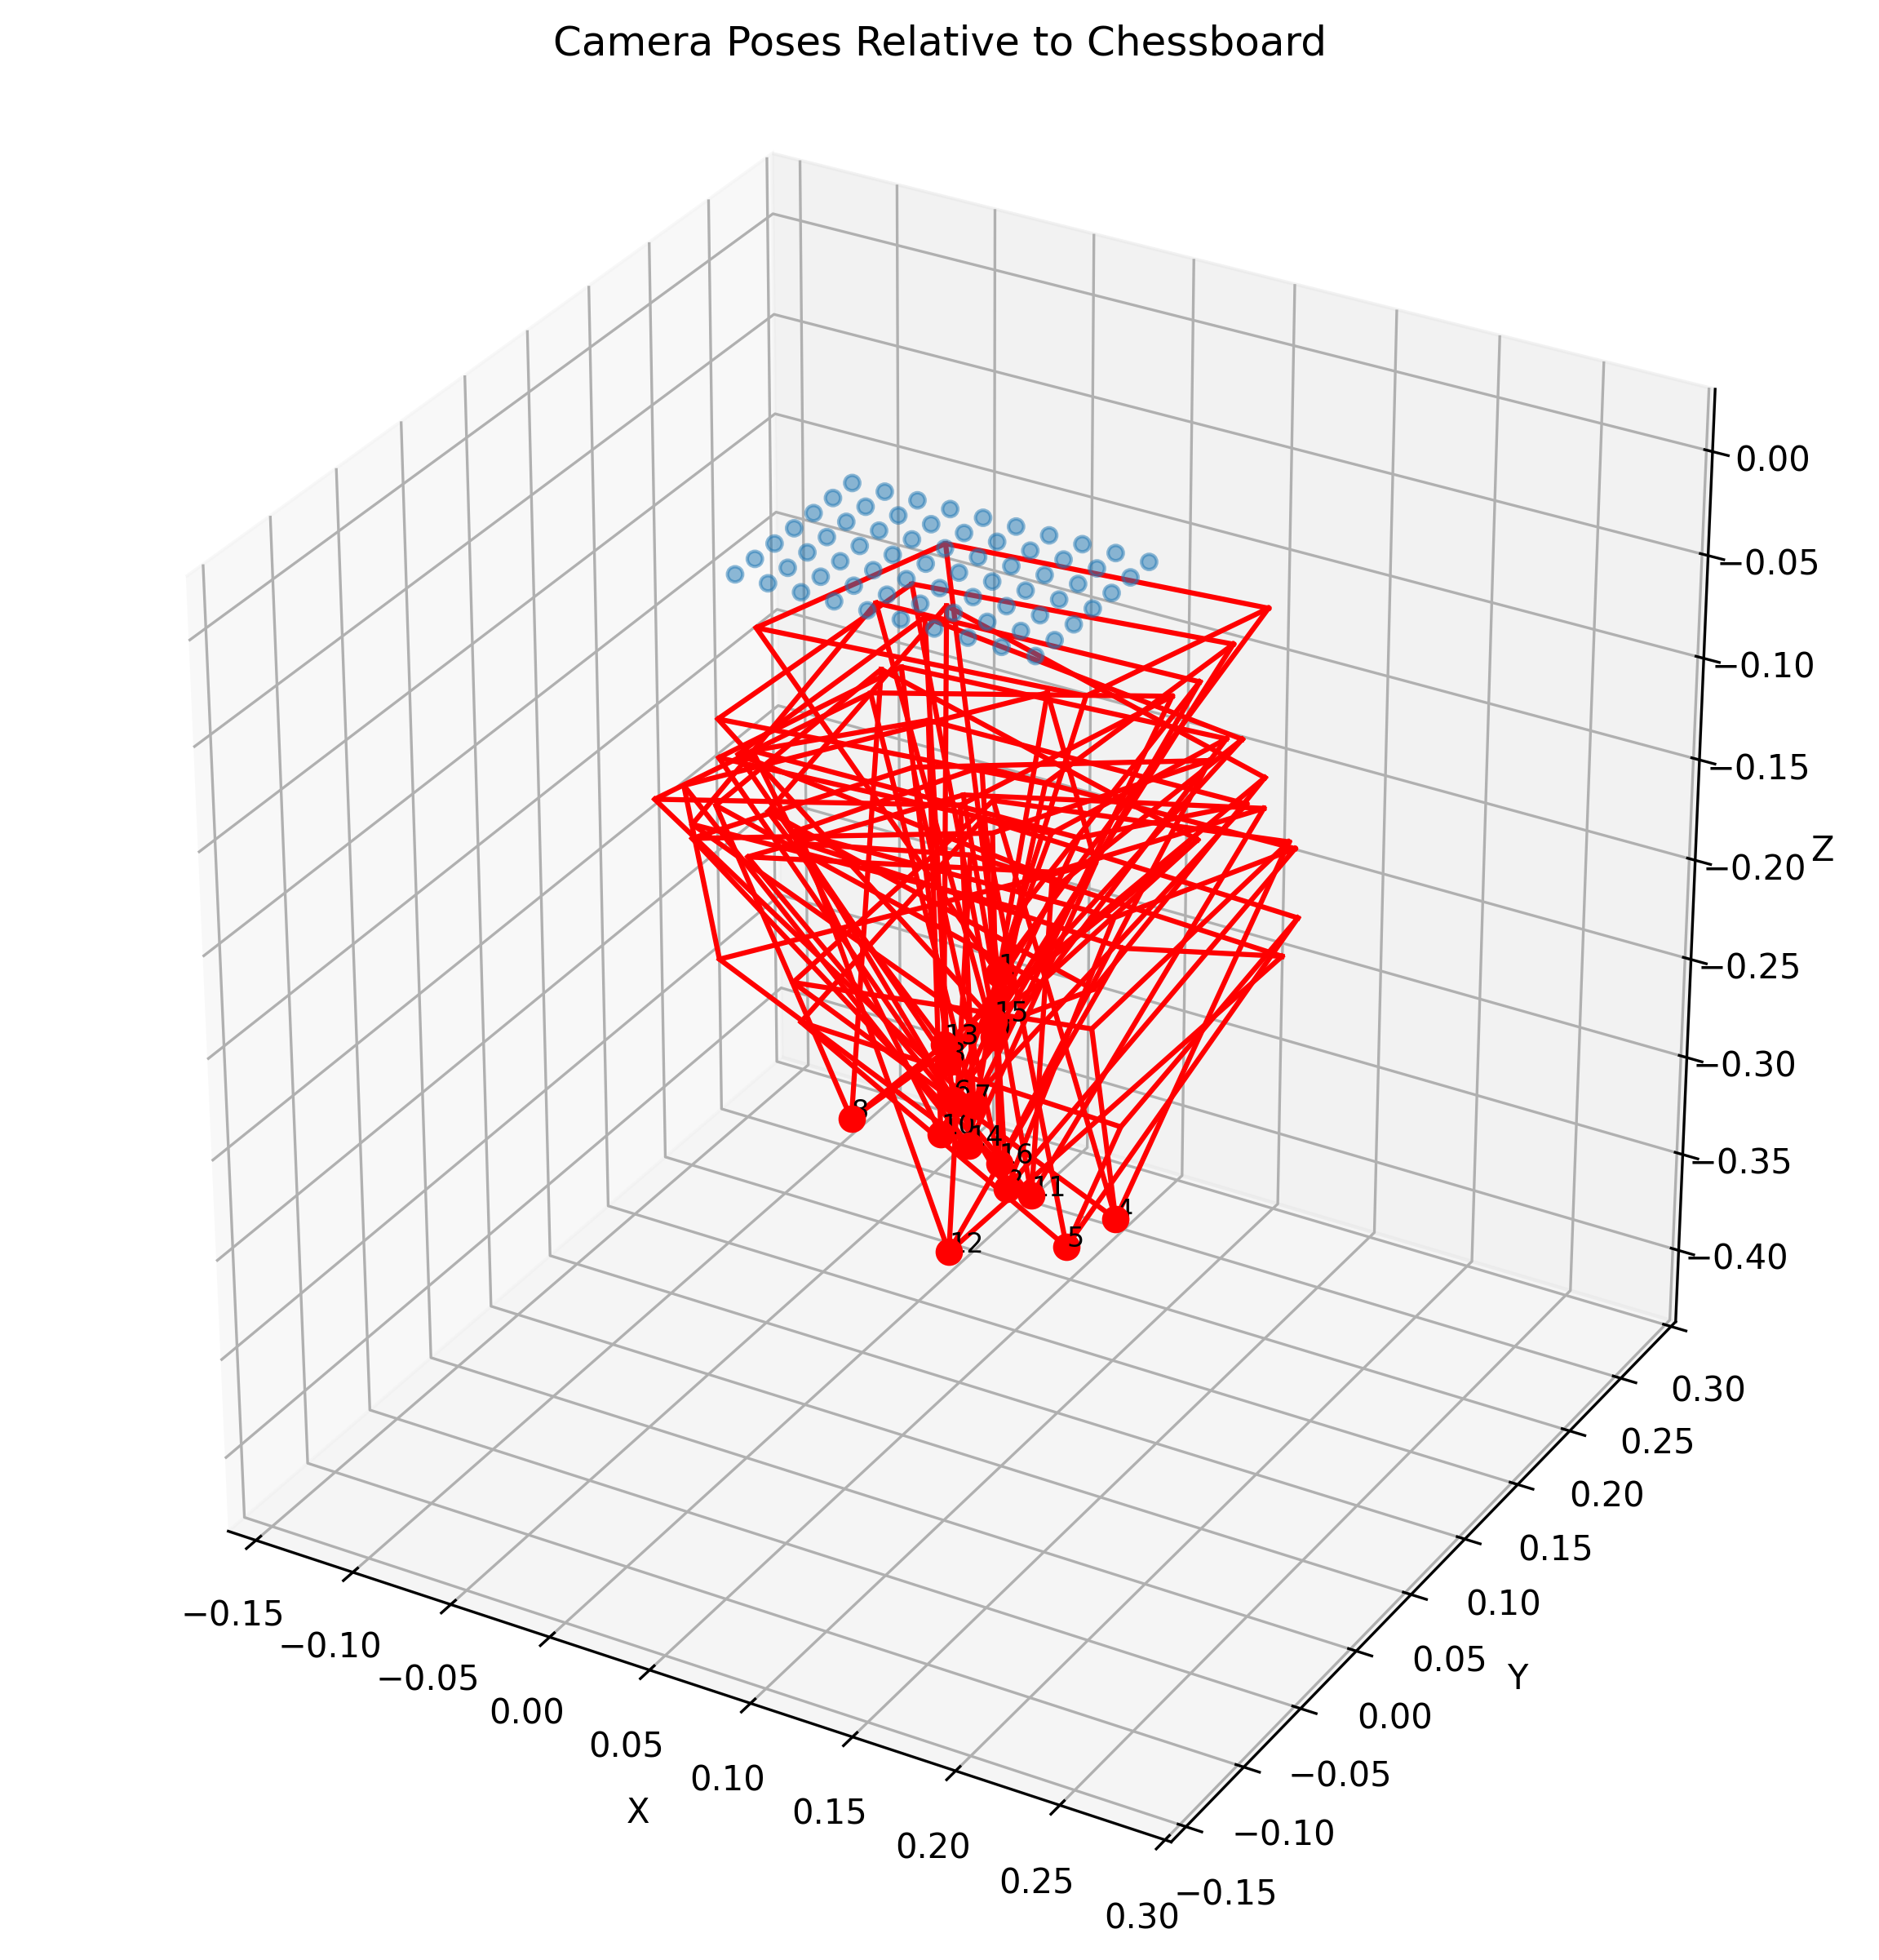
\includegraphics[width=0.8\textwidth]{images/camera_poses_3d.png}
	\caption{تصویرسازی سه‌بعدی موقعیت و جهت‌گیری دوربین نسبت به صفحه شطرنجی}
\end{figure}


در شکل ۲، شبکه شطرنجی به عنوان مرجع ثابت در نظر گرفته شده است. محورهای رنگی رسم شده در فضا نشان‌دهنده دستگاه مختصات محلی دوربین (شامل محورهای $X$، $Y$ و $Z$ دوربین) در لحظه ثبت هر تصویر هستند. 
تفسیر این نمودار حاکی از آن است که تصاویر از فواصل متنوع و زوایای دید گوناگون (شامل چرخش‌های مختلف حول محورهای مختصات) نسبت به الگو ثبت شده‌اند. این پراکندگی فضایی و تنوع زوایا برای یک کالیبراسیون مقاوم (\lr{Robust}) کاملاً ضروری است، زیرا الگوریتم کالیبراسیون برای تخمین دقیق پارامترهای اعوجاج لنز و ماتریس درونی به پرسپکتیوهای متفاوتی از یک الگوی مسطح نیاز دارد. پراکندگی مناسب این نقاط نشان می‌دهد که مجموعه داده جمع‌آوری شده برای رسیدن به خطای بازتولید (\lr{Reprojection Error}) پایین مناسب بوده است.


\newpage

\section{بخش دوم: بینایی استریو (\lr{Stereo Vision})}
در این بخش، هدف محاسبه نقشه عمق (\lr{Depth Map}) برای ۱۰۰ فریم از مجموعه داده هوایی \lr{Kagaru Airborne} و بازپروجکشن آن به فضای سه‌بعدی برای تولید ابر نقاط (\lr{Point Cloud}) است.

\subsection{استخراج پارامترهای مجموعه داده (\lr{Dataset Parameters})}
پارامترهای کالیبراسیون سیستم استریو شامل دو دوربین با رزولوشن $1280\times960$ پیکسل از مرجع دادگان استخراج گردید. ماتریس‌های درونی برای دوربین جلو (\lr{Front}) و عقب (\lr{Back}) و همچنین ماتریس انتقال و دوران بین آن‌ها مشخص شده است.

\subsubsection*{پارامترهای درونی (\lr{Intrinsic Parameters})}
\begin{itemize}
	\item \textbf{دوربین جلو (\lr{Front Camera}):}
	\begin{equation}
		K_{front} = \begin{bmatrix} 1641.99751 & 0 & 642.15139 \\ 0 & 1642.30964 & 470.34929 \\ 0 & 0 & 1 \end{bmatrix}
	\end{equation}
	ضرایب اعوجاج: $D_{front} = [-0.19978, 0.13511, -0.00007, -0.00005, 0.00000]$
	
	\item \textbf{دوربین عقب (\lr{Back Camera}):}
	\begin{equation}
		K_{back} = \begin{bmatrix} 1646.07299 & 0 & 620.74483 \\ 0 & 1645.39302 & 477.47527 \\ 0 & 0 & 1 \end{bmatrix}
	\end{equation}
	ضرایب اعوجاج: $D_{back} = [-0.20465, 0.18856, -0.00111, 0.00040, 0.00000]$
\end{itemize}

\subsubsection*{پارامترهای بیرونی استریو (\lr{Extrinsic Stereo Parameters})}
تبدیل هندسی انتقال ($T$) و دوران ($R$) از دوربین مبدأ به دوربین دوم به شرح زیر است:
\begin{equation}
	T = \begin{bmatrix} 6.09478 \\ -775.96641 \\ 7.36704 \end{bmatrix} (mm), \quad
	R = \begin{bmatrix} 0.9995 & -0.0035 & 0.0302 \\ 0.0031 & 0.9999 & 0.0112 \\ -0.0302 & -0.0111 & 0.9995 \end{bmatrix}
\end{equation}
بر اساس بردار انتقال، فاصله پایه خط مبنا (\lr{Baseline}) بین دو دوربین به طور تقریبی برابر با $B = 775.97$ میلی‌متر ($0.776$ متر) تخمین زده می‌شود.

\subsection{محاسبه نقشه عمق (\lr{Depth Map Estimation})}
با استفاده از توابع استریو در \lr{OpenCV} (مانند \lr{StereoBM} یا \lr{StereoSGBM})، ابتدا تصاویر کالیبره و اصلاح هندسی (\lr{Rectification}) می‌شوند تا خطوط اپی‌پولار (\lr{Epipolar Lines}) موازی گردند. سپس میزان اختلاف منظر یا دیسپاریتی (\lr{Disparity}) برای هر پیکسل محاسبه می‌شود:
\begin{equation}
	d = x_L - x_R
\end{equation}
پس از تعیین نقشه دیسپاریتی $d$، مقدار عمق حقیقی متناظر با هر پیکسل ($Z$) بر اساس رابطه عکس هندسی استخراج می‌گردد:
\begin{equation}
	\label{eq:depth}
	Z = \frac{f \cdot B}{d}
\end{equation}
که در آن $f$ میانگین فاصله کانونی دوربین‌ها و $B$ طول خط مبنا سیستم استریو است.

\subsection{بازپروجکشن سه‌بعدی به ابر نقاط (\lr{3D Back-Projection})}
با داشتن مقدار عمق هندسی $Z$ برای هر پیکسل تصویر در مختصات $(u,v)$، می‌توان مختصات سه‌بعدی حقیقی نقاط محیطی $(X,Y,Z)$ را در دستگاه مختصات دوربین با استفاده از رابطه عکس پروجکشن بازسازی کرد:
\begin{align}
	X &= \frac{(u - c_x) \cdot Z}{f_x} \\
	Y &= \frac{(v - c_y) \cdot Z}{f_y}
\end{align}
نتایج حاصل از این بخش برای تمام ۱۰۰ فریم به صورت توالی ویدئویی و فایل ابر نقاط ذخیره گردید که صحت بازسازی متریک محیط هوایی را نشان می‌دهد.







\section{ مراحل پیاده‌سازی بینایی استریو و بازسازی سه‌بعدی}

\subsection{مقداردهی اولیه پارامترها (\lr{Initialization})}	در این بخش، پارامترهای استخراج شده از وب‌سایت دادگان \lr{Kagaru} وارد کد محاسباتی می‌شوند:
	\begin{itemize}
	\item \textbf{ماتریس‌های درونی ($K$) و اعوجاج ($D$):} این ماتریس‌ها برای هر دو دوربین جلو (\lr{Front/Left}) و عقب (\lr{Back/Right}) با ابعاد تصویر $1280\times960$ پیکسل تعریف می‌گردند.
	\item \textbf{پارامترهای بیرونی ($R$ و $T$):} ماتریس دوران و بردار انتقال بین دو دوربین مقداردهی می‌شوند. از آنجا که هدف نهایی، دریافت نقشه عمق و تشکیل ابر نقاط با استاندارد متریک است، مقادیر میلی‌متری بردار انتقال (که دارای خط مبنا یا \lr{Baseline} در حدود $0.77$ متر است) بر $1000$ تقسیم شده‌اند تا تمامی واحدها در مقیاس متر تنظیم شوند.
\end{itemize}

\subsection{هم‌ترازی و تصحیح هندسی (\lr{Stereo Rectification})}	یکی از مهم‌ترین مفاهیم در بینایی استریو این است که یافتن نقاط متناظر یا مشابه در دو تصویر مختلف، یک پردازش دو‌بعدی بسیار سنگین از مرتبه $O(N^2)$ است. برای حل این مشکل تکنیکی و بهینه‌سازی فرآیند، از عملیات هم‌ترازی یا \lr{Rectification} استفاده می‌شود.
		تابع \lr{cv2.stereoRectify} از روی ماتریس‌های کالیبراسیون دوربین، تصاویری مجازی تولید می‌کند که گویی هر دو دوربین دقیقاً روی یک خط مستطیلی و موازی با صفحه تصویر (\lr{Image Plane}) قرار گرفته‌اند.
	
 با اعمال این الگوریتم، خطوط اپی‌پولار (\lr{Epipolar Lines}) کاملاً افقی و هم‌راستا می‌شوند. این بدان معناست که اگر به دنبال پیکسلی متناظر در تصویر چپ می‌گردیم، در تصویر راست نیازی به جستجوی دوبعدی نیست و تنها باید روی همان سطر افقی (جستجوی یک‌بعدی) به دنبال آن گشت.
	خروجی حیاتی دیگر این تابع، ماتریس $Q$ (\lr{Disparity-to-Depth Mapping Matrix}) است که برای تبدیل سیستم مختصات دوبعدی تصویر به فضای سه‌بعدی استفاده خواهد شد. در نهایت، توابع \lr{initUndistortRectifyMap} و \lr{remap} نقشه‌های هندسی انتقال پیکسل را ساخته و تصاویر کج و معوج اولیه را صاف، اصلاح و هم‌تراز می‌کنند.
	
\subsection{محاسبه نقشه اختلاف منظر (\lr{Disparity Map})}	اکنون که تصاویر کاملاً هم‌تراز شده‌اند، از الگوریتم تطابق بلوکی نیمه‌سراسری \lr{SGBM (Semi-Global Block Matching)} در کتابخانه \lr{OpenCV} استفاده می‌شود.
	
\textbf{تئوری اختلاف منظر (\lr{Disparity}):} اختلاف منظر یا دیسپاریتی ($d$) برابر است با اختلاف مختصات افقی یک شیء مشخص در تصویر چپ و راست که به صورت هندسی با رابطه $d=x_L-x_R$ بیان می‌شود. هرچه یک شیء در دنیای واقعی به دوربین نزدیک‌تر باشد، اختلاف منظر آن در تصاویر بیشتر است و هرچه دورتر باشد، این اختلاف منظر کمتر خواهد بود.
	الگوریتم \lr{SGBM} به جای مقایسه ساده پیکسلی، از بلوک‌های پیکسلی همسایه (در اینجا پنجره‌های $5\times5$) استفاده کرده و یک تابع جریمه انرژی سراسری را بهینه‌سازی می‌کند. این روش باعث می‌شود خروجی دارای نویز ساختاری کمتری بوده و مرزهای اشیاء به صورت دقیق‌تر استخراج شوند. خروجی این گام برای تمام فریم‌ها در قالب ویدئوی \lr{depth\_sequence.mp4} ذخیره می‌شود.
	
\subsection{بازتولید ابر نقاط سه‌بعدی (\lr{3D Reprojection})}	در گام نهایی، نقشهٔ اختلاف منظر دوبعدی باید به ساختار فضای هندسی سه‌بعدی (\lr{3D Point Cloud}) نگاشت شود. تابع \lr{cv2.reprojectImageTo3D} ماتریس نگاشت $Q$ را به عنوان ورودی دریافت کرده و ضرب ماتریسی زیر را برای تک‌تک نقاط اعمال می‌کند:
	\begin{equation}
	[X,Y,Z,W]^T=Q\cdot[u,v,d,1]^T
\end{equation}	این عملیات محاسباتی مستقیماً مقدار عمق واقعی ($Z$) را بر حسب متر (به دلیل مقیاس‌دهی اولیه بردار $T$ بر $1000$) به دست می‌دهد.
		در بخش پایانی الگوریتم، نقاطی که دارای عمق بی‌نهایت یا خارج از محدوده مجاز محاسباتی هستند فیلتر (\lr{Filter}) شده و حذف می‌گردند. سپس رنگ‌های اصلی استخراج‌شده از تصویر تصحیح‌شده به این نقاط تخصیص یافته و خروجی نهایی در قالب فایل‌های استاندارد \lr{.ply} ذخیره می‌شود. این فایل‌ها به راحتی در نرم‌افزارهای نمایش سه‌بعدی مانند \lr{MeshLab} قابل بارگذاری و تحلیل هستند.
	
\end{document}
